\documentclass[../mattg_ti-fi_lit-review.tex]{subfiles}


\subsection{History through Hall effects}

To understand where topological insulators (TIs) have come from, its useful to step back through the history of some significant physics phenomena. In this section I will discuss the quantum Hall effect, and how it's macroscopic behaviour can be explained by a Quantum effect called the Berry Phase. This will lead to the new ideas around 2005 of a Quantum spin Hall insulator, and eventually the concept of a 3D spin Hall material, now referred to as a 3D topological insulator.

\begin{figure}[H]\label{fig:ti_qh-trio}
	\centering
	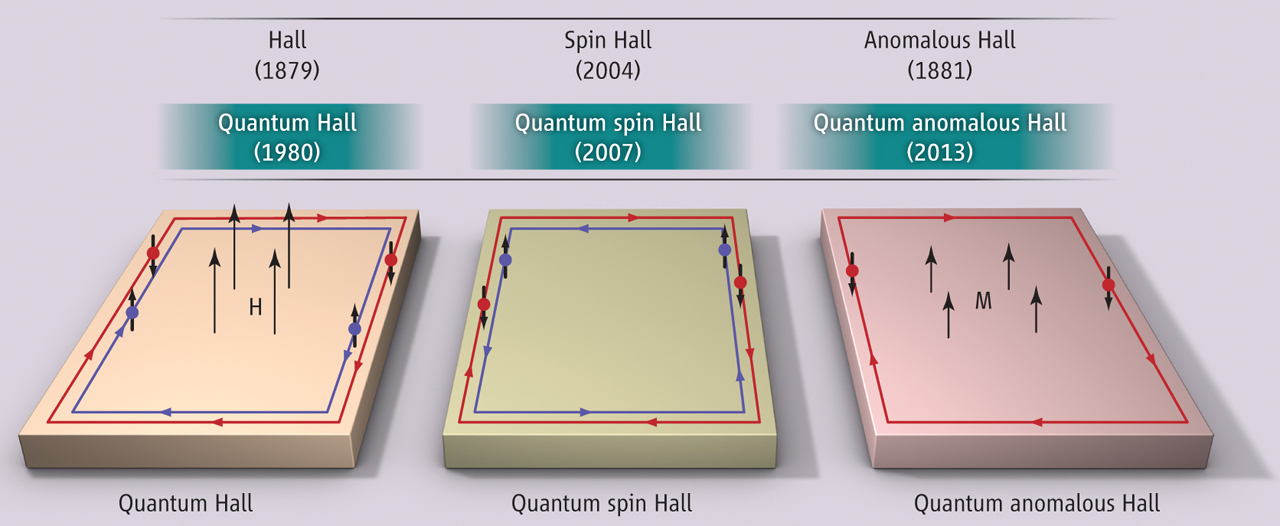
\includegraphics{ti_qh-trio.jpg}
	\caption{The three QH states discovered thus far. Source: Oh, Seongshik. \cite{oh_complete_2013}, Science Vol. 340, 153 (2013)}
\end{figure}

\subsubsection{Quantum Hall effect}\label{sec:QHE}

The quantum hall effect (QHE) was first discovered in MOSFET \footnote{Metal-oxide semiconductor field effect transistors} transistors 1980\cite{klitzing_new_1980}, through a 2 dimensional electron gas (2DEG) found at the interface of a bulk semiconductor and the gate oxide. The observation (Fig. \ref{fig:ti_qhe}) was that under strong magnetic fields, the longitudinal resistance disappeared, while the Hall resistance became quantised, following integer values of the fundamental factor $e^2/h$ (Eqn. \ref{eqn:qhe-conductivity}).  %TODO:Cite Klitzing et all 1980.

\begin{equation} \label{eqn:qhe-conductivity}
\sigma_{xy}=\nu \frac{e^2}{h}
\end{equation}

When introducing a magnetic field to materials, electrons bands undergo Landau quantisation. A physical understanding for this behaviour can be drawn from the quantisation of cyclotron orbits for charged particles in magnetic fields \footnote{The reason for cyclotron orbits is due to the single valued electron wavefunction, ie $\oint \vec{P}\cdot d\vec{r} = 2\pi N$}. Landau quantisation has the effect of creating new bands called "Landau Levels", that each posses large numbers of orbitals. The degeneracy of the level goes as 

\begin{equation}
	\text{Degeneracy} = \frac{B\times A}{\phi_0}=\frac{B\times A}{h/e}
\end{equation}

For some Fermi energy, the magnetic field can be chosen to an appropriate value to fill these Landau levels. 

\begin{figure}[]\label{fig:ti_qhe}
	\centering
	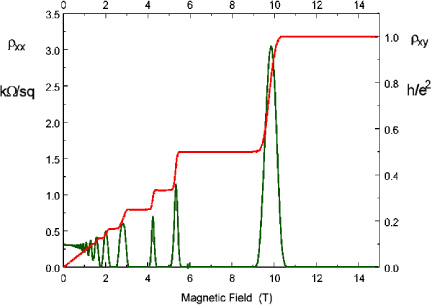
\includegraphics[width=\linewidth/2]{ti_qhe}
	\caption{The quantum Hall effect. $\rho_{xy}$ (red) is the Hall resistivity which obeys quantised values. $\rho_{xx}$ (green) vanishes at each Landau level, before peaking when scattering to bulk states can occur. 
	\\Courtesy of D.R. Leadley, Warwick University 1997.}
\end{figure}

The  QHE looks finely tuned. This is a result of electrons interacting at the edge, where there is a confinement of edge states \cite{haldane_topological_2018}. The edge states dominate transport when the Landau levels of the bulk are filled. Because they are dissipationless, the resistivity $\rho_{xx}$ of the system vanishes, before reaching the next Landau level, where scattering between bulk states can occur again. This is the hallmark of topological states, where there exists some states between different phases of matter.  %\footnote{Although unrelated to the Hall effect, get the pun? Haha.}

Thouless (who later received the Noble prize in 2016, before passing away in 2019), Kohmoto, Nightingale, and den Nijs (TKNN) \cite{thouless_quantized_1982} where interested in gapped bulk systems but with conductive edges and a periodic lattice potential. These systems had been argued for explaining the QHE by Laughlin\cite{laughlin_quantized_1981} and the integer effects had earlier been demonstrated theoretically by Hofstadter's Butterfly\cite{hofstadter_energy_1976}. TKNN recognised that \textbf{K} space maps to a non-trivial Hilbert space for the QHE; the space has a topology. This topology can be specified by the integer $\nu$ which also corresponds to the Hall conductance above in Eq. \ref{eqn:qhe-conductivity}. In particular, their calculations only depended on details of the wavefunctions of the bandstructure. 

While this system is not a coherent many-particle quantum ground state, it is fascinating in that it shows clear quantum and discrete properties in a macroscopic context. Other systems where we can observe such behaviour are few, including Bose Einstein Condensation, where many atoms condense into the same uniform quantum state, and superconductivity where the pairing of electrons (Cooper pairs) also produce a new phase of macroscopic quantum behaviour.

For the QHE to occur, the Landau quantisation opens gaps in the band structure of the material, and the chemical potential is situated within this gap. In a classical picture, the boundaries of the material cannot sustain these cyclotron orbit. Moving from the inside of the material to the outside requires a topological phase transition to an ordinary insulator, in which the bandgap needs to close, and so edge channels open in a \textbf{bulk-boundary correspondence}.

Note that the QHE does not preserve \textbf{time reversal} (TR) \textbf{symmetry}, as charge carriers experience different forces due to the magnetic field when their direction is inverted. The magnetic field breaks TR symmetry. This is explicit in the two degrees of freedom in the system; for an out of plane magnetic field, charge is separated into two lanes, and those channels move a particular direction, ie forward above for electrons, backward below for holes. Reversing the direction of carriers yields the same channels but switched, forward above for holes, backward below for electrons. 

\subsubsection{Berry Phase}\label{sec:berry}

In 1983, Barry Simon \cite{simon_holonomy_1983} recognised that the TKNN expression (that describes the QHE) is an integral over the curvature associated with the Berry phase on the Brillouin zone. This is fundamentally important to understanding that the QHE is a quantum phase effect, and has implications for more topological effects later in this review.

The \textbf{Berry Connection} is the expectation value of a Gradient operator of vector $\vec{R}$ acting on a wavefunction over some path  $\Gamma$ with positions $\vec{R}$. Physically it is the mechanism from getting one geometric space point to another, i.e. the change of parameters.
\begin{equation}
\vec{\mathcal{A}_n}(\vec{R}) = i\braket{\psi_n(\vec{R})|\nabla_{\vec{R}}|\psi_n(\vec{R})}
\end{equation}
This object has N parts, for each of the vector components. There's a different connection for every eigenstate, of every point in the space. 
It is a little more subtle than a vector - it transforms under gauge transformations. For an example wavefunction to include some additional phase factor (i.e. Gauge transformation), the wavefunction transforms as $\ket{\psi_n'(\vec{R})}=e^{-i\beta(\vec{R})}\ket{\psi_n(\vec{R})}$. This results in a change for the Berry connection:
\begin{equation}
\vec{\mathcal{A}_n'}(\vec{R}) = \vec{\mathcal{A}_n}(\vec{R}) + \nabla_{\vec{R}}\beta(\vec{R})
\end{equation}
So the ``connection" is that it transforms with the gradient of a function, like a vector potential.

\textbf{Berry Curvature} is the consequence or result of going from one set of starting parameters to the same set of parameters over some path (also called the Berry \textbf{connection}). The Schroedinger equation can be used to provide the Berry connection.  It turns out that through the parth evolution, the state can pick-up a phase factor, relative to the original starting state. This phase factor is also known as the Berry phase\cite{berry_quantal_1984}, and has consequences for the quantum mechanical properties of the system.

The \textbf{Berry Phase} is the integral
\begin{align}
\gamma_n(\Gamma) &= \int_\Gamma \vec{\mathcal{A}_n}(\vec{R})\cdot d\vec{R}
\end{align}
By changing the gauge of the Berry phase we can notice some properties that shift:
\begin{align}
\gamma'_n(\Gamma) &= \int_\Gamma \vec{\mathcal{A}_n}(\vec{R})\cdot d\vec{R} + \int_\Gamma \nabla_{\vec{R}}\vec{\beta} \cdot d\vec{R}\\
\implies \gamma'_n(\Gamma) &= \gamma_n(\Gamma) + \beta(R_f) - \beta(R_i)
\end{align}
It is not gauge invariant, which makes it difficult to measure. However, if the path begins \textbf{AND} ends in the same configuration point (ie, a closed loop) then the value is Gauge invariant! This imposes a few restrictions on the system to achieve a result.
\begin{itemize}
	\item Eigenstates have to be imaginary to achieve a non-zero Berry phase.
	\item If the path is 1D, then the integration cancels out to result in a zero Berry phase, again.
\end{itemize}

In 3D systems, the Berry phase over some path $\Gamma$ enclosing a surface $S$, then Stokes theorem can specify the \textbf{Berry curvature} $\vec{D}$ 
\begin{align}
\oint_\Gamma \vec{\mathcal{A}_n}\cdot d\vec{R} &= \oiint_S \left(\nabla\times\vec{\mathcal{A}}\right)\cdot d\vec{S}\\
\vec{D}&=\nabla_{\vec{R}}\times\vec{\mathcal{A}}_n(\vec{R})
\end{align}

The Berry phase is also useful for understanding other phenomena such as the Aharonov-Bohm effect.

%\paragraph{Aharonov–Bohm Effect}
%\textcolor{red}{Todo: Fill out some basic theory and why the Berry phase solves this problem} 
%TODO: Aharonov–Bohm effect

%\textcolor{red}{Show calculation of berry phase of the Bloch wave function calculated around the BZ boundary divided by 2 pi for the QHE / TKNN} 
%TODO - 


\subsubsection{Quantum spin Hall effect}\label{sec:QSHE}
The next large development towards topological insulators was the spin Hall was observed in 2004 by Kato \etal{} \cite{kato_observation_2004}, where for particular semiconductors a spin density was observed rather than a charge density, like in the regular Hall effect.
The origins for such an phenomenon are similar to that of the \hyperref[sec:QAHE]{anomalous Hall effect} in ferromagnets, sometimes being extrinsic, sometimes intrinsic. Intrinsically, the \textbf{Berry curvature} of the electronic valence-band Bloch wave functions result in spin-Hall effect. 

The spin Hall insulator was proposed by Murakami \etal \cite{murakami_spin-hall_2004}, where the Berry phase is finite implying a finite spin Hall conductivity. While this idea did not ``generate spin currents due to an absence of any electrons at the Fermi level"\cite{ando_topological_2013}, it allowed further exploration to find it quantised version, a quantum spin Hall (QSH) insulator \cite{bernevig_quantum_2006, kane_z_2005,kane_quantum_2005}.

In a real 1D system with spin, there are four degrees of freedom; Spin can move either direction, and can move forward and backward. This could be separated into two copies of the QH system - spin up moving forward with spin down moving backward at the top, and spin down moving forward with spin up moving backward on the bottom. This separation of states is referred to the quantum spin Hall effect (QSHE), however it requires a key ingredient to allow the separation of states to occur. In the QHE, it is the magnetic field that breaks time reversal symmetry. For QSH insulators, the essential ingredient is \hyperref[sec:SOC]{spin orbit coupling} (SOC).

An important step made by Kane and Mele\cite{kane_z_2005} was finding a ``topological invariant'' to characterise the QSH insulator states using an index. This index is called the $Z_2$ index. Topological invariants have appeared before. In the \hyperref[sec:QHE]{QHE}, the TKNN invariant $\mu$, where the quantised conductance is proportional to $\nu$. The consequence of the $Z_2$ index is it maps the parity of the number of times the 1D edge state crosses the Fermi level. An odd parity ensures the existence of an edge state and consequently the phase of a topological insulator. The result is significant in it shows how topological phases exist in band structures of insulators, and do not require  external magnetic fields breaking TRS like in the QHE \cite{ando_topological_2013}.

Whilst Kane and Mele used their SOC model to investigate the bandgap opening of graphene, SOC is very difficult to experimentally detect in graphene due to the low coupling strength, compared to that of heavier species. Berneveig et al. \cite{bernevig_quantum_2006}  (Zhang's group) instead proposed a $Z_2$ model for the band structure of mercury telluride (HgTe). They predicted a CdTe/HgTe/CdTe quantum well would give rise to the QSH effect, when the HgTe layer reached a certain critical thickness. Experimental observation was confirmed soon thereafter by K\"onig \cite{konig_quantum_2007}, who observed a quantised conductivity $\sigma_{xx}$ of $2e^2/h$, due to two conducting edges. They also observed the thickness dependence.

\subsubsection{Topological insulators}

By this time theorists (Moore \& Balents \cite{moore_topological_2007}, Fu, Kane and Mele\cite{fu_topological_2007}) had already leapt forward and predicted 3D systems that would exhibit quantum spin hall effects. It was at this point that the term ``topological insulator'' was first referred to\cite{moore_topological_2007}. Whilst these 3D systems cannot be called QSH insulators, they are an analogous 3D extension. The extension to 3D TIs results in no longer having one invariant to determine the topology of a system, but rather 4 separate invariants, for 16 classes of materials. Generally they could be separated into two groups - strong and weak 3D TIs.

The first prediction for a 3D TI was by Fu and Kane\cite{fu_topological_2007-2}. They predicted that the surface states of bismuth antimony (\bismuthantimony{}) could be observed by looking at angle resolved photo emission (ARPES, see \ref{sec:ARPES}). The signature for non-trivial topology was in observing surface states crossing the Fermi energy between two TR-invariant momenta \cite{fu_topological_2007-2} %TODO - Understand this last sentence and why ARPES can do this.
This was observed in the same system by Hsieh \etal \cite{hsieh_topological_2008}. 

%\subsection{Relevant theory and phenomena}
%\subsubsection{Topological field theory}
%In 2001 the QHE state was generalised to a 4D TR-invariant state by Zhang and Hu, and was generalised by to field theory by Bernevig \etal{}. It was also shown later by Zhang how the $Z_2$ topology could be described in this field theory, and be reduced to the 2D and 3D cases.
%
%Practically this is useful for describing electromagnetic response of TIs and predicting magnetoelectric effects, according to Ando's review \cite{ando_topological_2013}.

\subsection{Dirac fermions}
It is useful to consider the systems and behaviour of the particles in these materials, and as to why they draw much attention. Within graphene, mentioned earlier for the Kane and Mele SOC model \cite{kane_quantum_2005}, the 2D electron gas over the carbon honeycomb lattice creates interesting band structure features called ``Dirac cones". The carries occupying these band structure states behave according to a pseudo-relativistic Dirac equation, behaving differently to that of regular fermions in materials. Their physical behaviour mimics that of highly relativistic situations. 

\paragraph{Dirac fermion mass}:\\
Sometimes the charge carriers in graphene are called ``massless'' Dirac fermions - they behave analogous to relativistic particles with zero rest mass conforming to the Dirac equation \cite{novoselov_two-dimensional_2005-1}. This result comes from the observation of the fermions having a linear cyclotron mass with energy around the Dirac point's linear dispersion, effectively proving zero dependence on a "rest mass". Instead of their characteristic speed being the speed of light $c$, the Fermi velocity $v_F$ describes their motion. This has been verified in graphene.\\ %TODO Add verification reference.

Generally in semiconductors and other insulators, the electronic bands eitherside of the bandgap become quite flat with curvature in momentum space. The important of such features is reflected in the effective mass of carriers as the Fermi energy locally fills states at the band edge.
Historically, the effective mass of such carriers is calculated as \cite{kittel_introduction_nodate}
\begin{equation}
	m^* = \left(\frac{\partial E^2}{\partial^2k}\right)^{-1}
\end{equation}
For parabolic, isotropic bands, a local approximation to the effective mass is:
\begin{align}
	E(\textbf{k}) &= E_0 + \frac{\hbar^2\textbf{k}^2}{2m^*}\\
\end{align}
which satisfies the above calculation. In graphene however, the dispersion equation near the Dirac cones (the K and K' points) are similar to the Dirac equation:
\begin{align}
	E(\textbf{k}) \approxeq \hbar v_F \cdot \textbf{k}
\end{align}
If we apply the same effective mass equation, we arrive at:
\begin{align}
	m^* = \left(\frac{\partial v_F\cdot\textbf{k}}{\partial \textbf{k}^2}\right)^{-1} \to \infty
\end{align}
If the carriers were really so heavy, conduction would be very restricted in Graphene. Instead, a different method of calculating the effective mass has to be used  \cite{ariel_electron_2013} avoiding divergence.

\begin{align}
	m^*(E,\textbf{k}) &= \frac{p}{v_g} = h^2\textbf{k}\left(\frac{\partial E}{\partial \textbf{k}}\right)^{-1}\\
	&= h k \frac{1}{v_F} = h E \frac{1}{v_F^2}
\end{align}
This yields the mass proportional to the linear dispersion, just as $E=mc^2 \to m = E/c^2$, exhibiting relativistic behaviour.

\paragraph{Dirac particles in topological insulators}:\\
As pointed out by Ando\cite{ando_topological_2013}, Spin-orbit interactions and 3D ``massive'' Dirac theory have been known for a long time in bismuth research, which has also been a playground for its diamagnetism (different to Pauli paramagnetism \& diamagnetism). Wolff \cite{wolff_matrix_1964} showed that a 2 band bismuth model can be transformed into a 4-part Dirac Hamiltonian. 

It is interesting that both bismuth and another semi-metal antimony were used to produce the first 2D TI surface states in \bismuthantimony{} where 2D surface ``massless'' Dirac systems exist. A distinguishing property of massless Dirac fermions is the Berry phase of $\pi$, discussed earlier, which provides an absence of backscattering \cite{ando_berrys_1998}. The TI surface states are consequently electronically protected from some scattering.